\documentclass[tikz,margin=2mm]{standalone}

\newcommand*{\m}{\mathsf{m}}

\usetikzlibrary{trees,arrows}


\begin{document}

  		 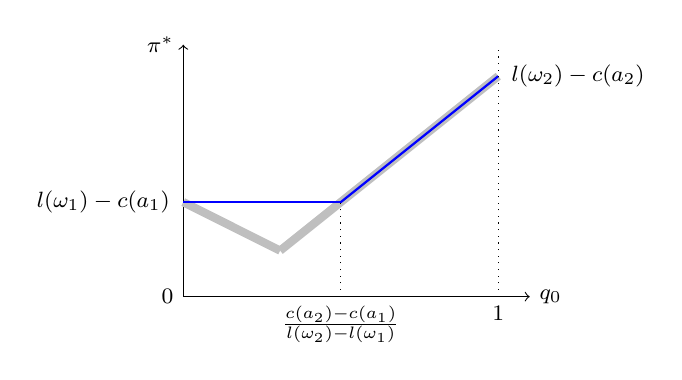
\begin{tikzpicture}[domain=0.001:1, scale=4, xscale=1,font=\footnotesize] 
  		%% vertices
    	\draw[->] (0,0) node[left]{$0$} -- (1.1,0) node[right] {$q_0$}; 
    	\draw[->] (0,0) -- (0,0.8) node[left] {$\pi^*$};

    	%% pi^m
    	\draw[line width=3pt, gray!50,] (1,0.7) node[right]{$\color{black}l(\omega_2) - c(a_2)$} -- (4/13, 3.2/13-0.1);	
    	\draw[line width=3pt, gray!50] (0,0.3) node[left]{$\color{black}l(\omega_1) - c(a_1)$} -- (4/13, 3.2/13-0.1);	


    	
    	%% quasiconcave
    	%% m
    	\draw[thick, blue] (0, 0.3) -- (0.5,0.3);	
    	%% s
    	\draw[thick, blue] (0.5,0.3)  -- (1,0.7) ;	
    	\draw[dotted] (0.5,0) node [below] {$\frac{c(a_2) - c(a_1)}{l(\omega_2) - l(\omega_1)}$} -- (0.5,0.3);



    	

    	%% labels
   	\draw[dotted] (1,0) node [below]{$1$}-- (1,0.8);
%    	\draw[->] (0.12,0.15) node [below, xshift=0.5cm] {$\bar p_1(q) - c(a_1)$}-- (0.15,0.2); 
%    	\draw[->] (0.8,0.36) node [below] {$\bar p_2(q) - c(a_2)$}-- (0.78,0.48); 
    	
       	\end{tikzpicture}
       	
\end{document}